\documentclass[letterpaper]{article}
    \usepackage{amsmath}
    \usepackage{tikz}
    \usepackage{epigraph}
    \usepackage{lipsum}
    \usepackage{float}
    \usepackage{glossaries}
    \usepackage{graphicx}
    \usepackage{imakeidx}
    \usepackage{hyperref}
    \graphicspath{{Images/}}
    \setcounter{tocdepth}{2}
    \makeglossaries
    \makeindex[columns=2, title=Alphabetical Index]
    \floatstyle{boxed}
    \restylefloat{figure}
    \renewcommand\epigraphflush{flushright}
    \renewcommand\epigraphsize{\normalsize}
    \setlength\epigraphwidth{0.7\textwidth}

    \definecolor{titlepagecolor}{cmyk}{1,.60,0,.40}

    \DeclareFixedFont{\titlefont}{T1}{ppl}{b}{it}{0.5in}

    \makeatletter
    \def\printauthor{%
        {\large \@author}}
    \makeatother
    \author{
        Sam Miller \\
       }

    % The following code is borrowed from:  https://tex.stackexchange.com/a/86310/10898

    \newcommand\titlepagedecoration{%
    \begin{tikzpicture}[remember picture,overlay,shorten >= -10pt]

    \coordinate (aux1) at ([yshift=-15pt]current page.north east);
    \coordinate (aux2) at ([yshift=-410pt]current page.north east);
    \coordinate (aux3) at ([xshift=-4.5cm]current page.north east);
    \coordinate (aux4) at ([yshift=-150pt]current page.north east);

    \begin{scope}[titlepagecolor!40,line width=12pt,rounded corners=12pt]
    \draw
      (aux1) -- coordinate (a)
      ++(225:5) --
      ++(-45:5.1) coordinate (b);
    \draw[shorten <= -10pt]
      (aux3) --
      (a) --
      (aux1);
    \draw[opacity=0.6,titlepagecolor,shorten <= -10pt]
      (b) --
      ++(225:2.2) --
      ++(-45:2.2);
    \end{scope}
    \draw[titlepagecolor,line width=8pt,rounded corners=8pt,shorten <= -10pt]
      (aux4) --
      ++(225:0.8) --
      ++(-45:0.8);
    \begin{scope}[titlepagecolor!70,line width=6pt,rounded corners=8pt]
    \draw[shorten <= -10pt]
      (aux2) --
      ++(225:3) coordinate[pos=0.45] (c) --
      ++(-45:3.1);
    \draw
      (aux2) --
      (c) --
      ++(135:2.5) --
      ++(45:2.5) --
      ++(-45:2.5) coordinate[pos=0.3] (d);
    \draw
      (d) -- +(45:1);
    \end{scope}
    \end{tikzpicture}%
    }




\begin{document}
\begin{titlepage}

	\noindent
	\titlefont Mumba\par
	\epigraph{A Project Mangement Solution\\ November 18, 2018}%
	{\textit{}\\ \textsc{}}
	\null\vfill
	\vspace*{1cm}
	\noindent
	\hfill
	\begin{minipage}{0.35\linewidth}
		\begin{flushright}
			\printauthor
		\end{flushright}
	\end{minipage}
	%
	\begin{minipage}{0.02\linewidth}
		\rule{1pt}{125pt}
	\end{minipage}
	\titlepagedecoration
\end{titlepage}
\tableofcontents
\pagebreak

\section{Introduction}

Mumba (https://mumba.azurewebsites.com) provides a simple no frills product management solution for small solo projects like those seen in university classes. My website is open to all and I hope that my project can be of use to myself and others in managing their projects and tasks. Anyone can register an account and use my application. Once the user has logged in they can boards which are collections of lists. They can then open the board and create tasks/cards in different lists to keep track of steps to complete a project. There currently is no user to user interactions, a board made by one user cannot be shared with any other user.

My Project is implemented as a full stack C\# ASP.Net Core application, I used the MVC pattern to dynamically manage the views returned to the users of my application. The buttons and interactions a user has with the website are controlled by one of the Four controller classes which will be detailed in the Description of Components section. The SQL server behind my web app is dynamically called to bring forth only the correct data that belongs only to the user who requested them. Each http request is routed to the proper controller's method for handling the request.

\section{Related Works}

The core functionality of Mumba is inspired by project boards (commonly known as  a kanban board) is commonly seen in Atlassian's Trello.com. Mumba is much simpler, there are not as many features as included in Trello, for example in Mumba's current state each board has 3 lists and only 3 lists, Trello dynamically allows creation and deletion of lists.

\section{System Architectural Design}
\begin{figure}[H]
  \centering
  \caption{The System Architecture}
  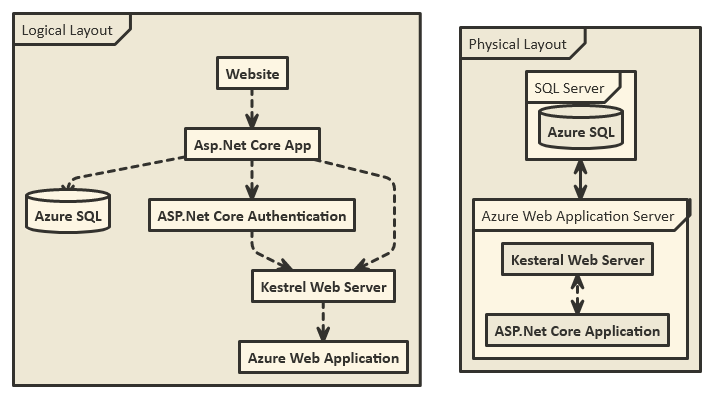
\includegraphics[scale=0.45]{Images/System}
\end{figure}
The system architecture follows the Model View Controller model of web design. The application was deployed across two Azure instances one is the platform as a service Web App Container that hosts my ASP.Net Core MVC web application, the second instance is a Windows Server Running an SQL Server. With a Azure web application a domain name is automatically registered, in my case my website can be reached at https://mumba.azurewebsites.net.

The views of my websize use Razor (HTML + C\# functionality) pages as a base and materialize css: https://materializecss.com as the basis for the look and feel of my website. The models are made to represent any non static entity that could be used by Mumba, the views are used by the controllers to display the data and forms to the user and build the functionality of the application.

SQL was chosen for the database system due to the general benefits of Relational Databases for persistant storage of data and its ability to integrate with ASP.Net Core web application. The bellow ER diagram was developed with the needs of Mumba in mind.

\begin{figure}[H]
  \centering
  \caption{The ER Model}
  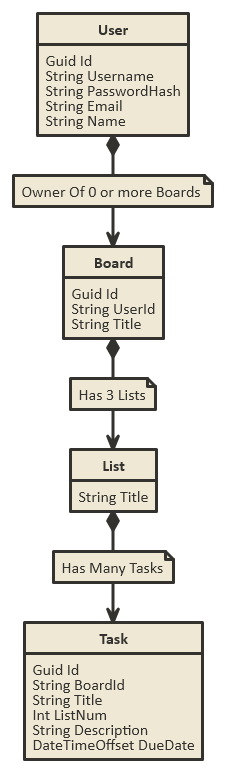
\includegraphics[scale=0.5]{Images/ER}
\end{figure}

The assumptions and constraints:
\begin{itemize}
  \item All Guids are non-nullable
  \item Lists are static
\end{itemize}

This model was migrated to relational tables for use in a SQL database that is used by the controllers to retrieve and modify the data. The four tables resulting from my models are shown below, there are several tables used by the Microsoft Identity package that are not included.
\subsection{Relational table: AppUsers}
The AppUsers table stores user account information. The primary key is the Guid Id and Guid's are inherantly unique.
\begin{center}
\begin{tabular}{|c|c|c|c|}
  \hline
  \underline{ID} & UserName & Email & Password Hash \\
  Guid & String & String & string\\
  \hline
\end{tabular}
\end{center}

\subsection{Relational table: Boards}
The boards table stores all of the Boards created by users. The primary key is an automatically generated Guid. The User ID is a foriegn key that is the AppUser.ID of the creating user. The Title is a string that will be displayed on the boards listing and at the top of the board.
\begin{center}
  \begin{tabular}{|c|c|c|}
    \hline
    \underline{ID} & UserID & Title \\
    Guid & String & String\\
    \hline
  \end{tabular}
  \end{center}
\subsection{Relational table: Tasks}
The Tasks table stores all tasks created by users. The primary key is an automatically generated GUid. The BoardId is a foriegn key that attatches a task to a board. The ListNum determines which of the three lists the task is placed in.
\begin{center}
  \begin{tabular}{|c|c|c|c|c|c|c|}
    \hline
      \underline{Id} & BoardId & ListNum & Title & Description & DueDate & Open \\
      Guid & string & int & string & string & DateTime & bool \\
    \hline
  \end{tabular}
  \end{center}

\section{Detailed Description of Components}

The following is a detailed Description of each functional componet of the Mumba application, I have organized them by the Controller class that handles the requesst and response for each call. Each handled http request is directed to a controller and then a specific method of that controller. In most cases a new view is called but a small handful of cases do not return a view.
Invalid calls will result in a error page being displayed, and in order to view information beyond the register and login page one must be logged in.

\subsection{Account}
The Account controller handles session management and login/log out functionality.

\subsubsection{Login}
Takes a LoginRequest model that is generated by taking the username and password from the login views form and it will also grab a boolean value based off of the checkbox for session remembrance. It will then attempt to log the user in using the loginrequest model, if the request fails the user is redirected to the login page. If the login request succeeds then the user is sent to the BoardsController's All method. The following screenshot is of the Login page.


\begin{figure}[H]
  \centering
  \caption{The Login View}
  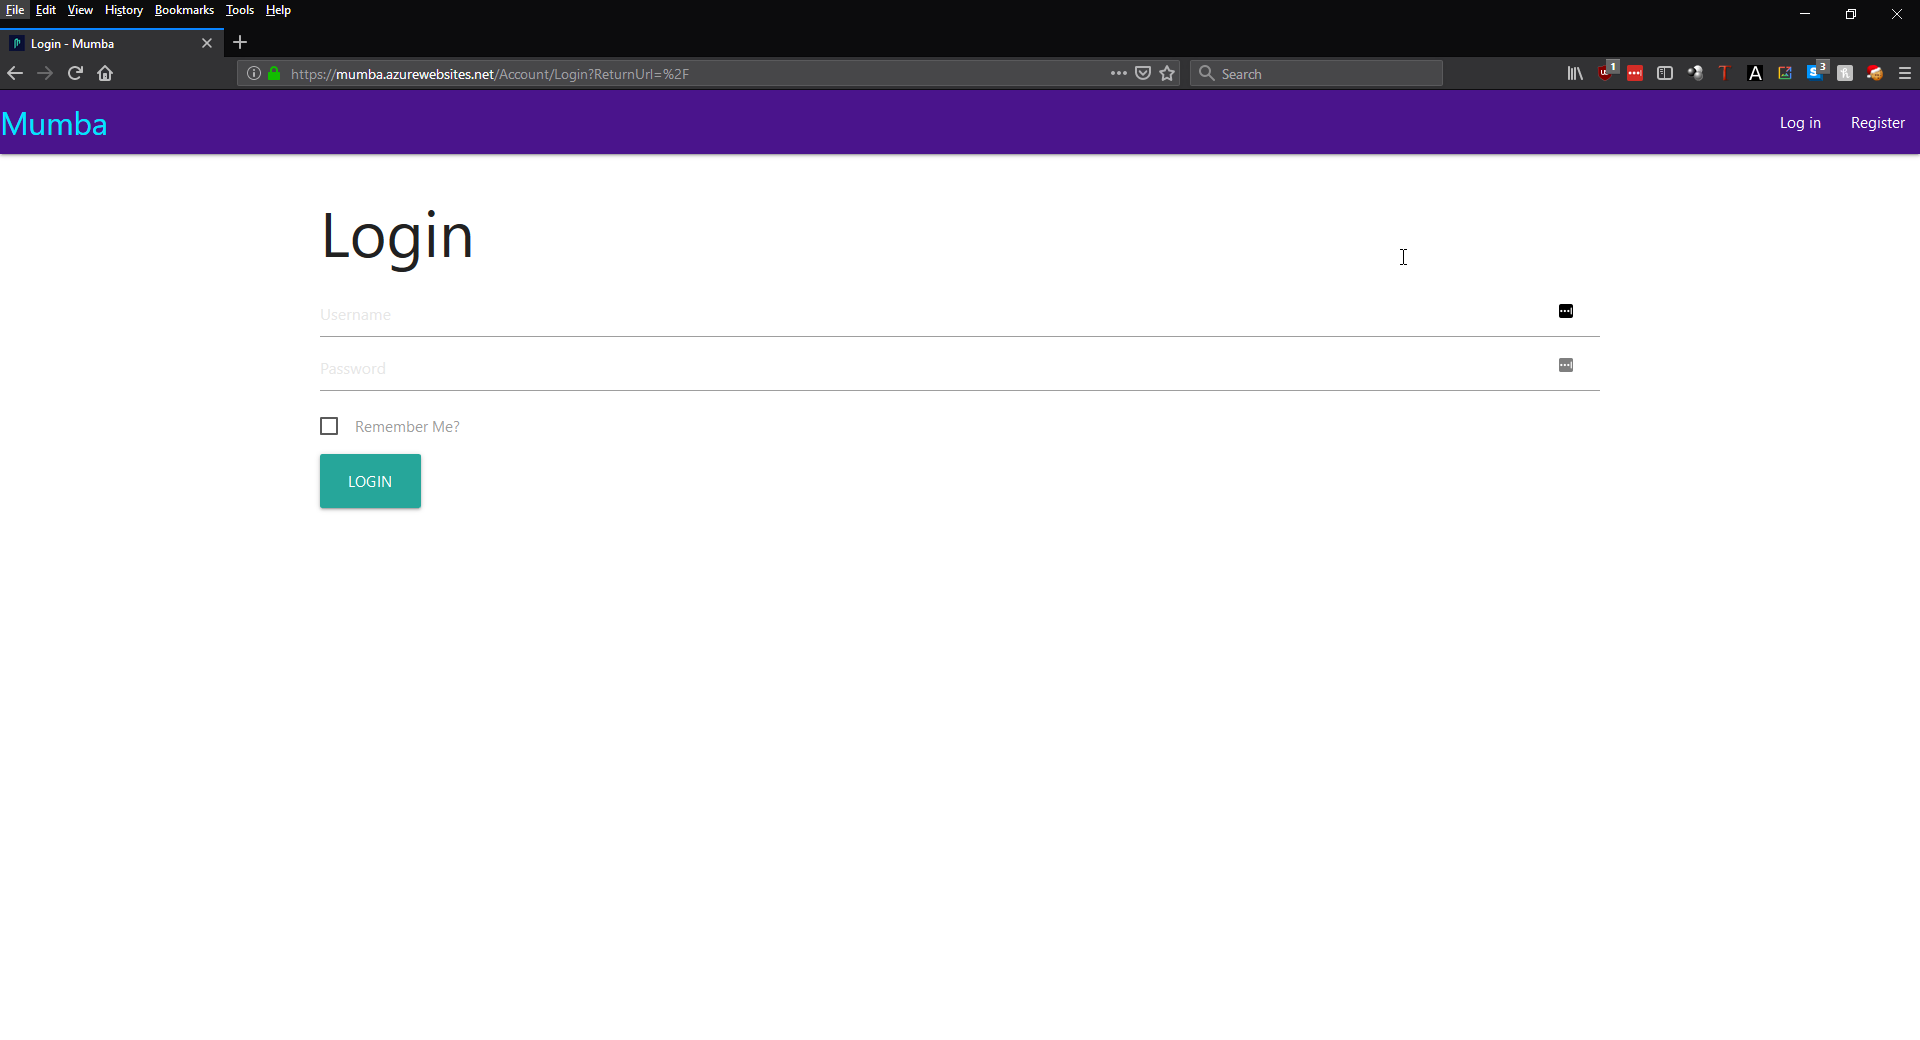
\includegraphics[scale=0.2]{Images/Login}
\end{figure}

\subsubsection{Logout}
This method ends a users session when the logout button in the navbar is pressed and redirects the browser to the login page.

\pagebreak
\subsection{User}

The user controllers main function is to handle the creation of accounts. 

\subsubsection{AddUser}
The AddUserFunction handles the creation of Users from the UserRegistration page.
The information from the Registration pages form is loaded into a NewAppUser model and then passed to the userManager to have the account registered to the database. The following screenshot is of the User Registration (AddUser) view.

\begin{figure}[H]
  \centering
  \caption{The User Registration View}
  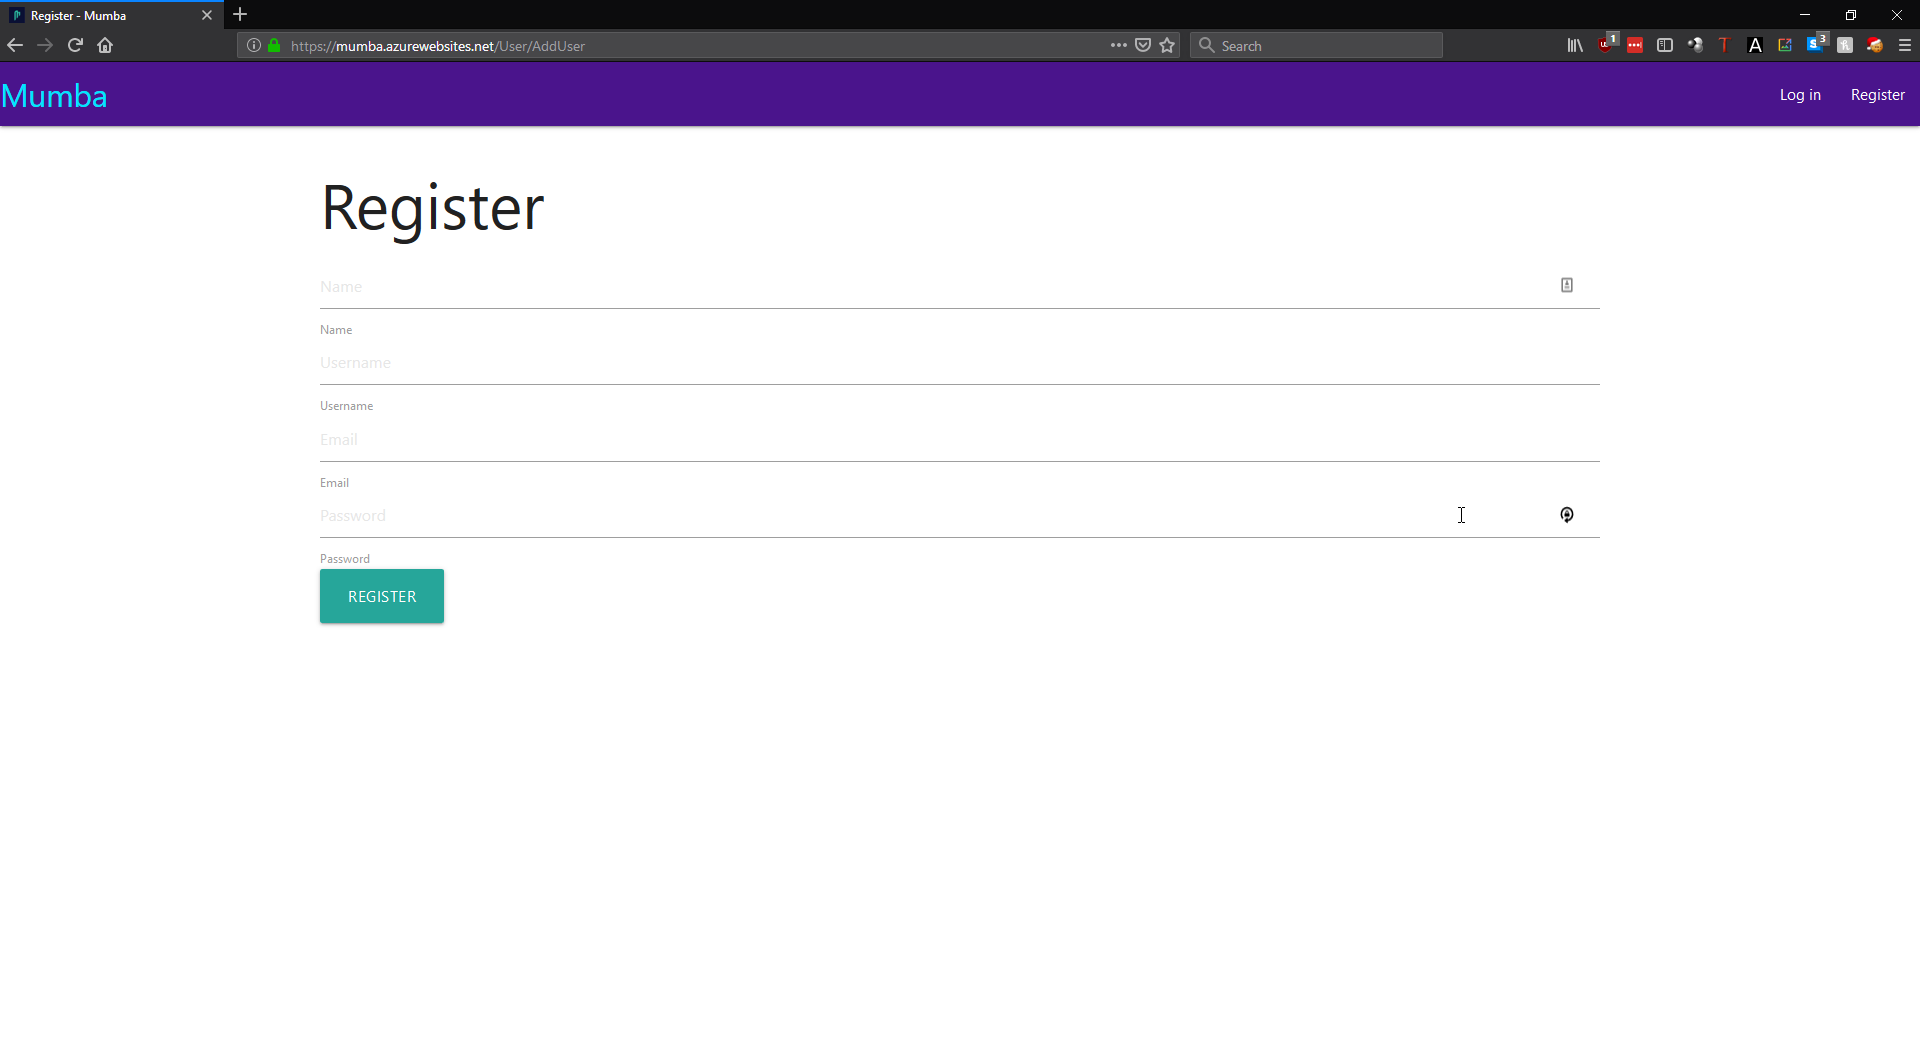
\includegraphics[scale=0.2]{Images/Register}
\end{figure}

\pagebreak
\subsection{Boards}

The BoardsController handles all tasks associated with Creating / Displaying / Editing / Deleteing boards.

\subsubsection{All}

The All Boards function is the deafault landing page for users when they first login. The function retreives all boards that have the UserID matching the currently logged in user's ID and then displays them in the All Boards view. The view below is what a user with out any boards will see, and the image below that is a user with many boards.

\begin{figure}[H]
  \centering
  \caption{The All Boards View}
  \includegraphics[scale=0.2]{Images/"Your Boards"}
\end{figure}

\begin{figure}[H]
  \centering
  \caption{The All Boards View With Many Boards}
  \includegraphics[scale=0.2]{Images/"BoardWMC"}
\end{figure}

\pagebreak

\subsubsection{Open}

The Open Board function handles opening a single board from the list of boards. It takes the Guid of the board from the url that is passed by the open board button and returns a view  genertated by getting all of the Tasks associated with the board divided into 3 lists and parsed into the card views. The default view pictured blelow of a board with no tasks created. The view below shows a board with many tasks.

\begin{figure}[H]
  \centering
  \caption{The Open Board View}
  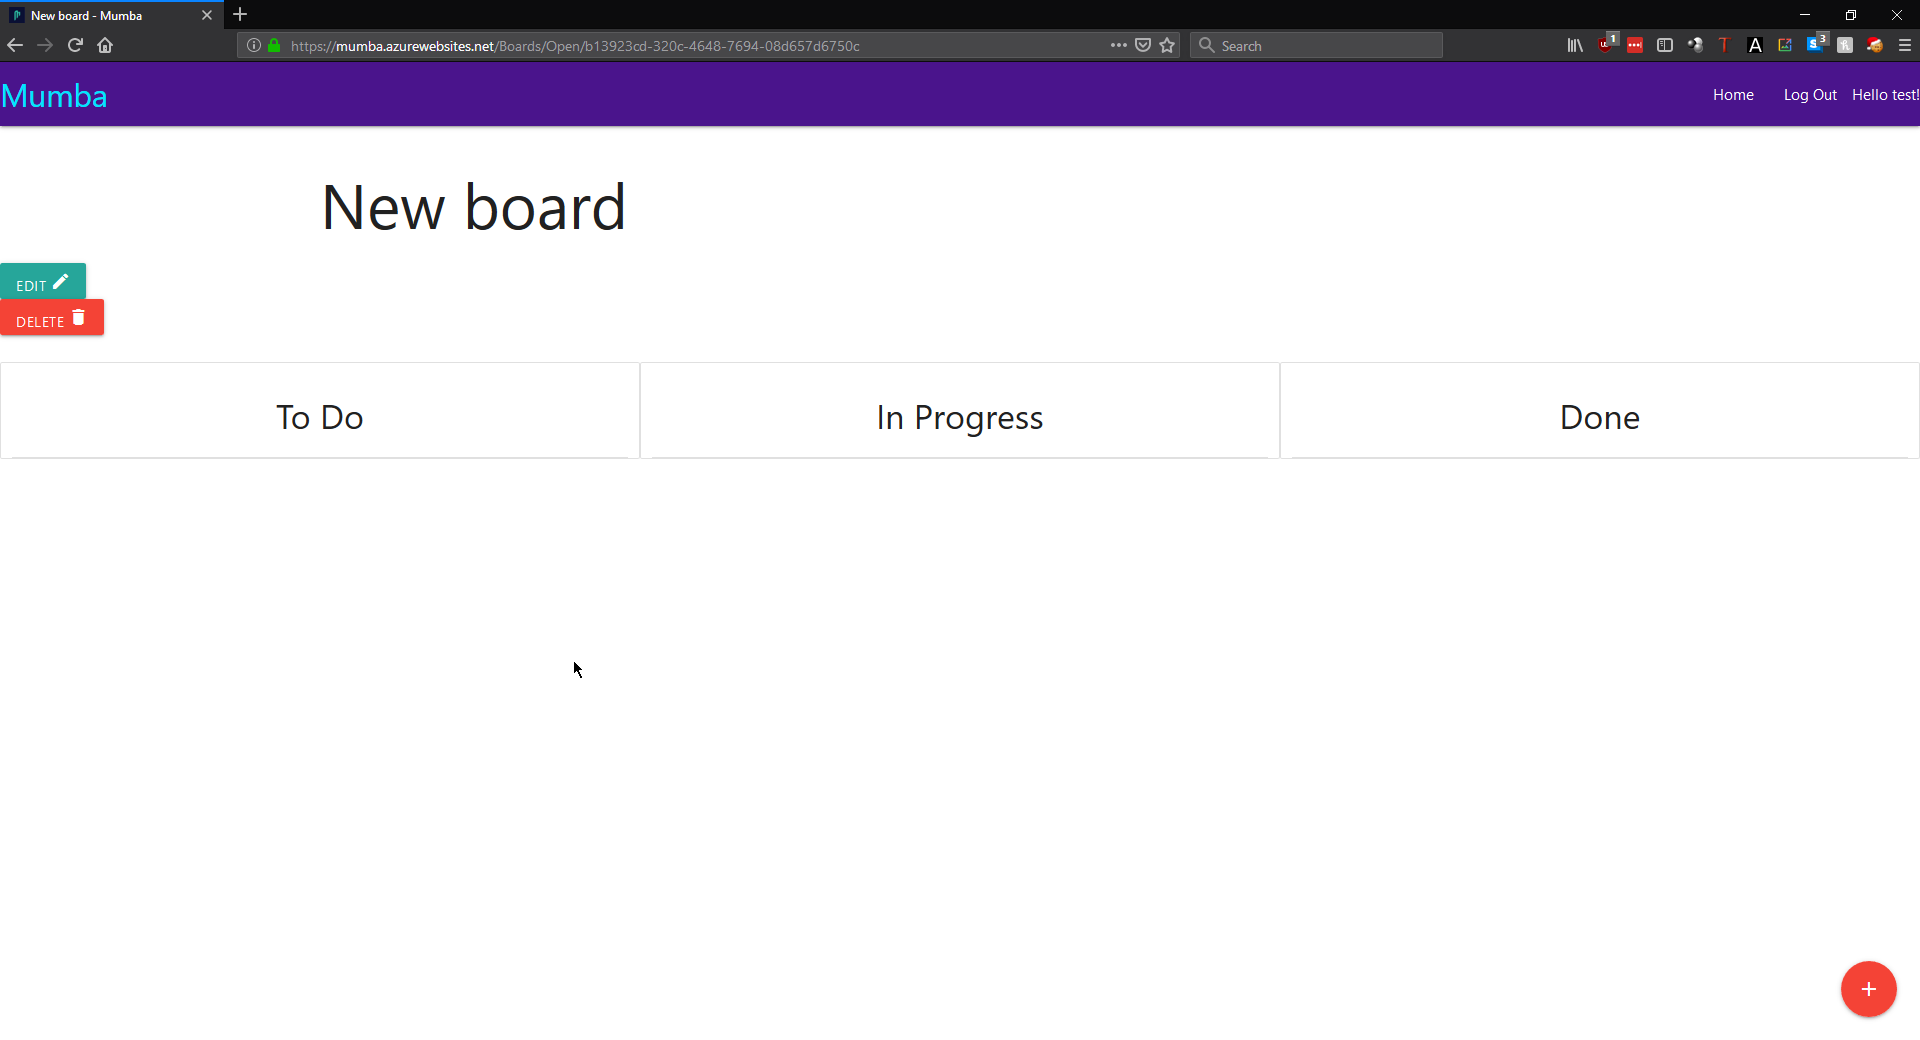
\includegraphics[scale=0.2]{Images/BlankBoard}
\end{figure}

\begin{figure}[H]
  \centering
  \caption{The Open Board View with Many Tasks}
  \includegraphics[scale=0.2]{Images/"BoardWMT"}
\end{figure}
\pagebreak
\subsubsection{Add}

The Add Board function handles the creation of Boards. When a user is brought to the Add Board View they supply a title and click the create button. The controller then adds the users ID and a created Guid to the model and adds it to the database. The board Creation form is shown below.

\begin{figure}[H]
  \centering
  \caption{The Board Creation View}
  \includegraphics[scale=0.2]{Images/"Add Board"}
\end{figure}


\subsubsection{Edit}

The Edit Board function handles the editing of Boards. A Guid of a board is supplied by the action generated by the edit button, and the user is given the ability to change the title of the board. Upon clicking the Update button the change is saved to the database by the functions post method.

\begin{figure}[H]
  \centering
  \caption{The Board Edit View}
  \includegraphics[scale=0.2]{Images/"Edit Board"}
\end{figure}

\subsubsection{Delete}
  The Delete function removes the Board and all cards associated with the board from the database.
\pagebreak

\subsection{Tasks}
The TasksController handles all tasks associated with Creating / Displaying / Editing / Deleteing Tasks.
\subsubsection{Open}
The open function handles displaying a detailed view of the task as pictured below. From here a task can be edited or deleted.

\begin{figure}[H]
  \centering
  \caption{The Task Open View}
  \includegraphics[scale=0.2]{Images/"Task_ Task"}
\end{figure}


\subsubsection{Add}
The Add Task function handles the creation of a new task from a form. The Title and Description are supplied by the user and the application adds the generated Guid for the Task and the Id of the board the task was created in before saving the Task to the database.
\begin{figure}[H]
  \centering
  \caption{The Add Task View}
  \includegraphics[scale=0.2]{Images/"Add Task"}
\end{figure}

\subsubsection{Edit}

The Edit Tasks function handles the editing of Tasks. A Guid of a task is supplied by the action generated by the edit button, and the user is given the ability to change the title and description of the task. Upon clicking the Update button the change is saved to the database by the functions post method.

\begin{figure}[H]
  \centering
  \caption{The Task Edit View}
  \includegraphics[scale=0.2]{Images/"Edit Task"}
\end{figure}


\subsubsection{Delete}
The delete function removes the task from the Database.

\pagebreak
\section{Conclusion}
The final implementation of Mumba delivers a fully functional web application hosted at https://mumba.azurewebsites.net that meets the goals of providing a simple and easy to use project management solution. The service is very secure, with security as a choice from the very beginning. Using the Microsoft Identity package the website handles session management and data security natively. I used the CSS grid to create the many different elements of my pages, and in doing so made my website responsive, it will function and look good on any screen size. The main areas that Mumba could be improved are the following:
\begin{itemize}
  \item One: Allow the dynamic creation/deletion/naming of lists within boards.
  \item Two: Create a method of sharing boards between two or more users to allow collaborative projects to be managed in Mumba
\end{itemize}
Once both of these features are implemented Mumba would be in a state that I would consider feature complete, anything else that would be added would just be extra.
\pagebreak
\section{Index}
\listoffigures

\end{document}
